\section{Gestion de la numérotation des éléments et du maillage}\label{sec:mesh}
Votre travail consistera dans cette partie à identifier les n\oe uds (ou points) présents dans l'élément de référence et faire le lien avec les noeuds présents dans le maillage. 

\subsection{Définition du maillage}
Dans le cas 1D, un maillage est défini comme un ensemble de points et d'arêtes liant ces points. Celui-ci est défini par 2 tableaux :
\begin{itemize}
	\item Un premier tableau, \texttt{vertices}, définit l'ensemble des extrémités des segments.
	\item Un deuxième tableau, \texttt{edges}, définit l'ensemble des segments du maillage. Il s'agit d'un tableau de connectivité orienté : chaque colonne représente un segment ; toute la colonne vaut 0 sauf en deux lignes, valant -1 pour le point de départ du segment et 1 pour le point d'arrivée.
\end{itemize}

Un exemple est donné figure \ref{fig:maillage_1D}.

\begin{figure}[!h]
\begin{minipage}{0.49\textwidth}
    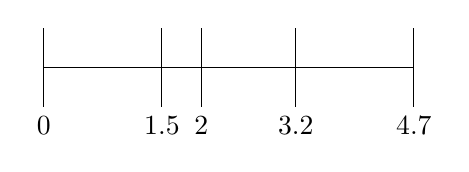
\begin{tikzpicture}
    \foreach \xm/\xp in {0/1.5, 1.5/2, 2/3.2, 3.2/4.7} {
        \draw (\xm,0) -- (\xp,0);
	\draw (\xm, 0.5) -- (\xm, -0.5) node[below] {\xm};
    }
    \draw (4.7, 0.5) -- (4.7, -0.5) node[below] {4.7};
    \end{tikzpicture}	
\end{minipage} \hfill
\begin{minipage}{0.5\textwidth}
\texttt{vertices} = (0, 1.5, 2, 3.2, 4.7)\\
\texttt{edges} = $\begin{pmatrix} 
-1 \\
 1 & -1 \\
   &  1 & -1\\
   &    &  1 & -1\\
   &    &    &  1
\end{pmatrix}$
\end{minipage}
\caption{Exemple d'encodage d'un maillage 1D.}
\label{fig:maillage_1D}
\end{figure}


\begin{mdframed} 
\textbf{Tâche 1} Complétez la fonction \texttt{generate\_mesh\_structured} dans le fichier \texttt{Mesh1D.jl}. Cette fonction doit prendre en entrée les extrémités d'un intervalle $[a,b]$ ainsi que le nombre de sous-intervalles, et renvoie un \texttt{Mesh1D} encodant le maillage associé.
Vous devrez également remplir le tableau \texttt{entity\_counts} en accord avec la documentation de \texttt{Mesh1D}.
La fonction \texttt{spzeros} vous permet d'initialiser un tableau sparse de type \texttt{SparseMatrixCSC} ; allez voir sa documentation.
\end{mdframed}
\begin{mdframed}[linecolor=ForestGreen] 
{\color{ForestGreen} \textbf{Test 1}} Écrivez deux tests unitaires permettant de vous assurer que les maillages sont bien construits.
\end{mdframed}

\subsection{Définition des n\oe uds dans l'élément de référence}
La méthode des éléments finis se base sur une intégration effectuée sur un élément de référence. Ici, on prendra comme élément de référence l'intervalle $[-1,1]$, même si le code autorise d'autres intervalles de référence (à prendre en compte dans votre code !).
Sur cet élément de référence, on définit un ensemble de n\oe uds équirépartis servant à définir les polygones de base servant à définir la base de l'espace fonctionnel sur lequel on résout les EDP.
Ce sont en ces n\oe uds qu'on définit les polynômes suivant la règle $\hat{P}_i(x_j) = \delta_{ij}$.
Nous avons déjà vu certains exemples en TD :
\begin{itemize}
	\item L'espace des polynômes de degré 1 est de dimension 2 (les deux coefficients dans $ax+b$), il faut donc 2 degrés de libertés et donc deux n\oe uds sur l'élément de référence, situés aux extrémités de l'intervalle.
	\item L'espace des polynômes de degré 2 est de dimension 3 (les trois coefficients dans $ax^2+bx+c$), il faut donc 3 degrés de libertés et donc trois n\oe uds sur l'élément de référence : deux aux extrémités, un au milieu de l'intervalle.
\end{itemize}

On voit qu'ainsi, pour définir un espace de polynômes de degré $k$ (noté $\mathbb{P}_k$), il nous faut $k+1$ n\oe uds sur l'élément de référence. En les supposant équirépartis sur l'intervalle, on peut facilement calculer la position de chaque n\oe ud dans l'intervalle.
Ceci est illustré dans la figure \ref{fig:noeuds_1D}.
\begin{figure}[!h]
\begin{subfigure}{0.3\textwidth}
\centering
   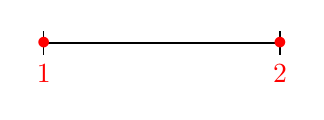
\begin{tikzpicture}[scale = 1.5]
   \draw (-1, 0) -- (1, 0);
   \draw (-1, -0.1) -- (-1, 0.1);
   \draw ( 1, -0.1) -- ( 1, 0.1);
   \draw[color=red] (-1,0) node {$\bullet$};
   \draw[color=red] (-1,-0.1) node[below] {1};
   \draw[color=red] (1,0) node {$\bullet$};
   \draw[color=red] (1,-0.1) node[below] {2};
   \end{tikzpicture}
   \caption{Degré 1}	
\end{subfigure}
\begin{subfigure}{0.3\textwidth}
\centering
   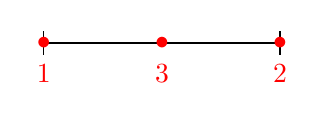
\begin{tikzpicture}[scale = 1.5]
   \draw (-1, 0) -- (1, 0);
   \draw (-1, -0.1) -- (-1, 0.1);
   \draw ( 1, -0.1) -- ( 1, 0.1);
   \draw[color=red] (-1,0) node {$\bullet$};
   \draw[color=red] (-1,-0.1) node[below] {1};
   \draw[color=red] (1,0) node {$\bullet$};
   \draw[color=red] (1,-0.1) node[below] {2};
   \draw[color=red] (0,0) node {$\bullet$};
   \draw[color=red] (0,-0.1) node[below] {3};
   \end{tikzpicture}	
   \caption{Degré 2}	
\end{subfigure}
\begin{subfigure}{0.3\textwidth}
\centering
   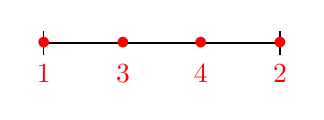
\begin{tikzpicture}[scale = 1.5]
   \draw (-1, 0) -- (1, 0);
   \draw (-1, -0.1) -- (-1, 0.1);
   \draw ( 1, -0.1) -- ( 1, 0.1);
   \draw[color=red] (-1,0) node {$\bullet$};
   \draw[color=red] (-1,-0.1) node[below] {1};
   \draw[color=red] (1,0) node {$\bullet$};
   \draw[color=red] (1,-0.1) node[below] {2};
   \draw[color=red] (-0.33,0) node {$\bullet$};
   \draw[color=red] (-0.33,-0.1) node[below] {3};
   \draw[color=red] (0.33,0) node {$\bullet$};
   \draw[color=red] (0.33,-0.1) node[below] {4};
   \end{tikzpicture}	
   \caption{Degré 3}	
\end{subfigure}
\caption{Position des n\oe uds, ainsi que leur numérotation, dans l'élément de référence suivant le degré de l'élément fini.}
\label{fig:noeuds_1D}
\end{figure}

On définit, par la même occasion, une numérotation sur les n\oe uds. Pour des raisons pratiques lors de la numérotation globale, ces n\oe uds sont numérotés par entité (une entité étant soit un point, de dimension 0, soit une arête, de dimension 1). 
Ainsi, on commence par numéroter les n\oe uds associés aux points (les extrémités de l'intervalle) puis on numérote les n\oe uds à l'intérieur de l'intervalle, associés à l'arête.


\begin{mdframed} 
\textbf{Tâche 2} Implémentez la génération des n\oe uds de Lagrange dans la fonction \texttt{LagrangeElement1D} dans \texttt{FiniteElement.jl}. Cela se fait en une ligne avec les fonctions \texttt{range} et \texttt{collect}. 
Laissez de côté l'attribut \texttt{basis\_coeffs}, rempli par un de vos collègues.
Implémentez également la construction du dictionnaire \texttt{entity\_nodes} donnant la liste des n\oe uds associés à chaque entité. 
Regardez bien la structure de ce dictionnaire ainsi que la documentation de \texttt{FiniteElement1D}.
En reprenant la numérotation dans la figure \ref{fig:noeuds_1D}, vous devriez obtenir :
\begin{itemize}
	\item Degré 1 : 
   \texttt{entity\_nodes[0] = [1 => [1], 2 => [2]]},\\
   \texttt{entity\_nodes[1] = []}
	\item Degré 2 : 
   \texttt{entity\_nodes[0] = [1 => [1], 2 => [3]]},\\
   \texttt{entity\_nodes[1] = [1 => [2]]}
	\item Degré 3 : 
   \texttt{entity\_nodes[0] = [1 => [1], 2 => [4]]},\\
   \texttt{entity\_nodes[1] = [1 => [2,3]]}
\end{itemize}
\end{mdframed}
\begin{mdframed}[linecolor=ForestGreen] 
{\color{ForestGreen} \textbf{Test 2}} Écrivez au moins deux tests unitaires permettant de vous assurer que les \texttt{FiniteElement1D} sont bien construits. Pensez à tester plusieurs configurations pour tester chaque attribut que vous générez dans la tâche 2.
\end{mdframed}

\subsection{Numérotation globale}
Dans la section précédente, nous avons défini une numérotation locale pour chaque n\oe ud. Chaque n\oe ud définit un coefficient dans l'approximation éléments finis d'une fonction $u$ ; par exemple, en $\mathbb{P}_2$, on définit une fonction sur l'élément $E_k$ par $u(x) = u_0^k P_0(x) + u_m^k P_m(x) + u_1^k P_1(x)$. 
Les coefficients $u_i^k$ sont définis élément par élément (ou en 1D, sous-intervalle par sous-intervalle), certains de ces coefficients étant communs à deux éléments (pensez aux coefficients associés à l'extrémité commune à deux sous-intervalles).
Afin de distinguer chaque coefficient dans le maillage, la numérotation locale ne suffit plus. 
On doit donc définir une numérotation globale de ces coefficients, dans l'ensemble du maillage mais qui est basée sur la numérotation locale dans l'élément de référence (et notamment, sur l'organisation par entité).

Il existe plusieurs numérotations possibles (qui peuvent être optimisées pour des raisons de performances de calcul, afin de limiter les sauts dans la mémoire). Nous allons ici rester sur une numérotation simple.
Comme on se base sur la numérotation locale, on va garder la même organisation : on commence par numéroter tous les n\oe uds associés aux points du maillage (la dimension 0) puis on numérote les n\oe uds associés aux arêtes. 
Cette logique donne par exemple la numérotation illustrée Figure \ref{fig:num_globale} (voyez la correspondance qu'on peut y voir avec le degré 2 dans la Figure \ref{fig:noeuds_1D}).

\begin{figure}[!h]
\centering
   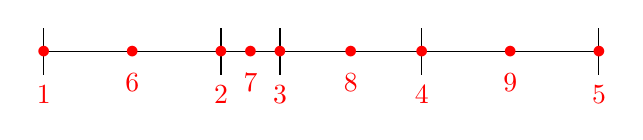
\begin{tikzpicture}[scale = 1.5]
    \foreach \i/\xm/\xp in {1/0/1.5, 2/1.5/2, 3/2/3.2, 4/3.2/4.7} {
        \draw (\xm,0) -- (\xp,0);
	\draw (\xm, 0.2) -- (\xm, -0.2);
   	\draw[color=red] (\xm,0) node {$\bullet$};
        \draw[color=red] (\xm,-0.2) node[below] {\i};
    }
    \draw (4.7, 0.2) -- (4.7, -0.2);
   \draw[color=red] (4.7,0) node {$\bullet$};
   \draw[color=red] (4.7,-0.2) node[below] {5};
   \foreach \i/\xm/\xp in {6/0/1.5, 7/1.5/2, 8/2/3.2, 9/3.2/4.7} {
	\pgfmathsetmacro\result{0.5*(\xm + \xp)}
       \draw[color=red] ((\result,0.) node {$\bullet$};
       \draw[color=red] ((\result,-0.1) node[below] {\i};
   }
   \end{tikzpicture}	
   \caption{Numérotation globale, dans un cas d'EF de degré 2. Dans la cellule 3, le n\oe ud d'indice local 3 devient le n\oe ud d'indice global 8 (ou écrit autrement, l'indice local (3,3) devient l'indice global 8).
		Le n\oe ud d'indice global 4 est à la fois l'indice local (3,2) et l'indice local (4,1).}	
   \label{fig:num_globale}
\end{figure}

On a donc une formule qui permet de calculer le premier indice associé à l'entité de dimension $d$ pour le sous-intervalle $i$ :
	\[G_{d,i} = \left(\sum_{\delta < d} N_\delta E_\delta\right) + iN_d\]
où $N_d$ est le nombre de n\oe uds associé à chaque entité de dimension $d$, et $E_d$ le nombre d'entité de dimension $d$ dans le maillage. 
Dans l'exemple de la figure \ref{fig:num_globale}, on aurait donc $N_0 = 1$, $N_1 = 1$, $E_0 = 5$, $E_1 = 4$.

Grâce à cette construction, il existe une correspondance entre les n\oe uds définis sur l'élément de référence et les n\oe uds définis sur chaque sous-intervalle.
Cette correspondance est stockée dans un tableau de dimension 2 de taille (nombre de sous-intervalles $\times$ nombre de n\oe ud par sous-intervalle). 
Dans chaque ligne, on respecte l'ordre dans lequel sont rangés les n\oe uds dans l'élément de référence : on liste d'abord les indices liés aux extrémités du sous-intervalle (entité de dimension 0), puis on liste les indices liés aux arêtes (entité de dimension 1).
Ainsi, pour l'exemple dans la figure \ref{fig:num_globale}, on devrait avoir le tableau suivant :
\[\mathtt{cell\_node\_mappings} = \begin{pmatrix}
1 & 2 & 6\\
2 & 3 & 7\\
3 & 4 & 8 \\
4 & 5 & 9
\end{pmatrix}\]

\begin{mdframed} 
\textbf{Tâche 3} Terminez la définition du constructeur \texttt{FiniteElementSpace1D} dans \texttt{FiniteElementSpace.jl}. Le travail consiste principalement à compléter la définition de \texttt{cell\_node\_mappings}.
Vous pourriez pour cela vous intéresser à la fonction \texttt{cumsum} de \texttt{Julia} ainsi qu'à la fonction \texttt{adjacency} définie dans \texttt{Mesh1D.jl} qui renvoie les indices des points associés à l'arête numéro $i$ (voir la documentation). 
Attention : la structure de données ne suppose pas forcément que les points et les arêtes sont rangés dans l'ordre croissant !
\end{mdframed}
\begin{mdframed}[linecolor=ForestGreen] 
{\color{ForestGreen} \textbf{Test 3}} Écrivez au moins un test unitaire permettant de vous assurer que \texttt{cell\_node\_mappings} est bien construit.
\end{mdframed}

